%To compile as handout, use
%pdflatex "\def\ishandout{1} \input{filename.tex}"
%Defaults to non-handout mode (with slide reveals)
\ifdefined\ishandout
  \documentclass[handout]{beamer}
\else
  \documentclass{beamer}
\fi
 
\usepackage{econ103slides} 

\date{Lecture 24}


\begin{document} 




%%%%%%%%%%%%%%%%%%%%%%%%%%%%%%%%%%%%%%%%

\begin{frame}[plain]
	\titlepage 
	

\end{frame} 


%%%%%%%%%%%%%%%%%%%%%%%%%%%%%%%%%%%%%%%%

\begin{frame}
\begin{center}
	\huge Regression -- Part II
\end{center}
\end{frame}
%%%%%%%%%%%%%%%%%%%%%%%%%%%%%%%%%%%%%%%%
\begin{frame}
\frametitle{Recall: ``Best Fitting'' Line Through Cloud of Points}
\begin{figure}
	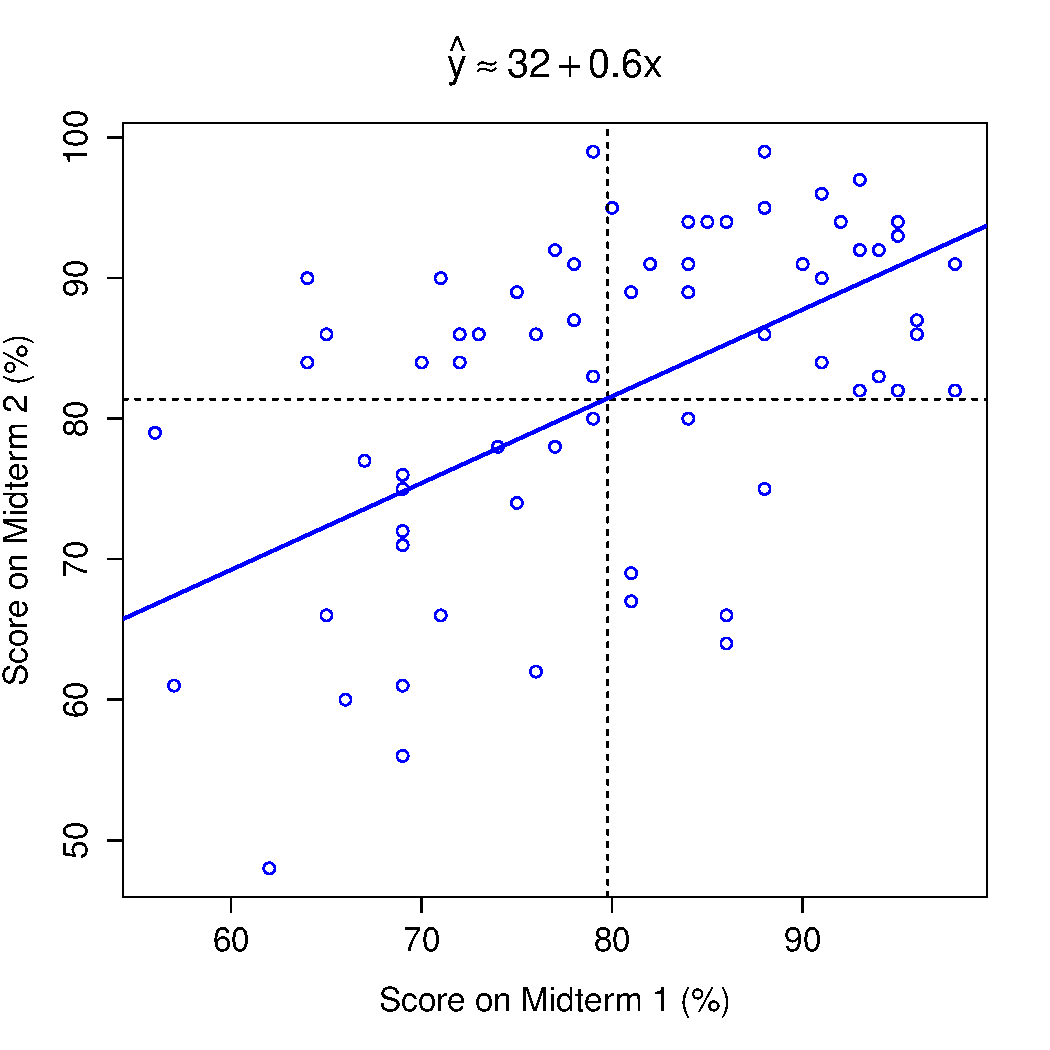
\includegraphics[scale = 0.48]{./images/midterms5}
\end{figure}
\end{frame}
%%%%%%%%%%%%%%%%%%%%%%%%%%%%%%%%%%%%%%%%
\begin{frame}
\frametitle{Recall: Regression as a Data Summary}
\begin{block}{Linear Model}
$\hat{y} = a + b x$
\end{block}
\begin{block}{Choose $a,b$ to Minimize Sum of Squared Vertical Deviations}
$\displaystyle\sum_{i = 1}^n d_i^2 = \sum_{i=1}^n (y_i - a - b x_i)^2$
\end{block}

\begin{block}{The Prediction}
Predict score $\hat{y} = a + b x$ on second midterm for someone with score $x$ on first.
\end{block}

\end{frame}
%%%%%%%%%%%%%%%%%%%%%%%%%%%%%%%%%%%%%%%%
\begin{frame}
\frametitle{Recall: Regression as a Data Summary}
	\begin{block}{Problem}
	$$\min_{a,b}  \sum_{i=1}^n (y_i - a - b x_i)^2$$
\end{block}
\begin{block}{Solution}
	\begin{eqnarray*}
		b &=& \frac{\sum_{i=1}^n \left(y_i - \bar{y}\right)\left(x_i - \bar{x} \right)}{\sum_{i=1}^n \left(x_i - \bar{x}\right)^2} = \frac{s_{xy}}{s_x^2} =  r\frac{s_y}{s_x}\\ \\
		a &=& \bar{y} - b\bar{x}
	\end{eqnarray*}
\end{block}
\end{frame}
%%%%%%%%%%%%%%%%%%%%%%%%%%%%%%%%%%%%%%%%
\begin{frame}
\frametitle{Beyond Regression as a Data Summary}
\small
Based on a sample of Econ 103 students, we made the following graph of handspan against height, and fitted a linear regression:
\begin{center}
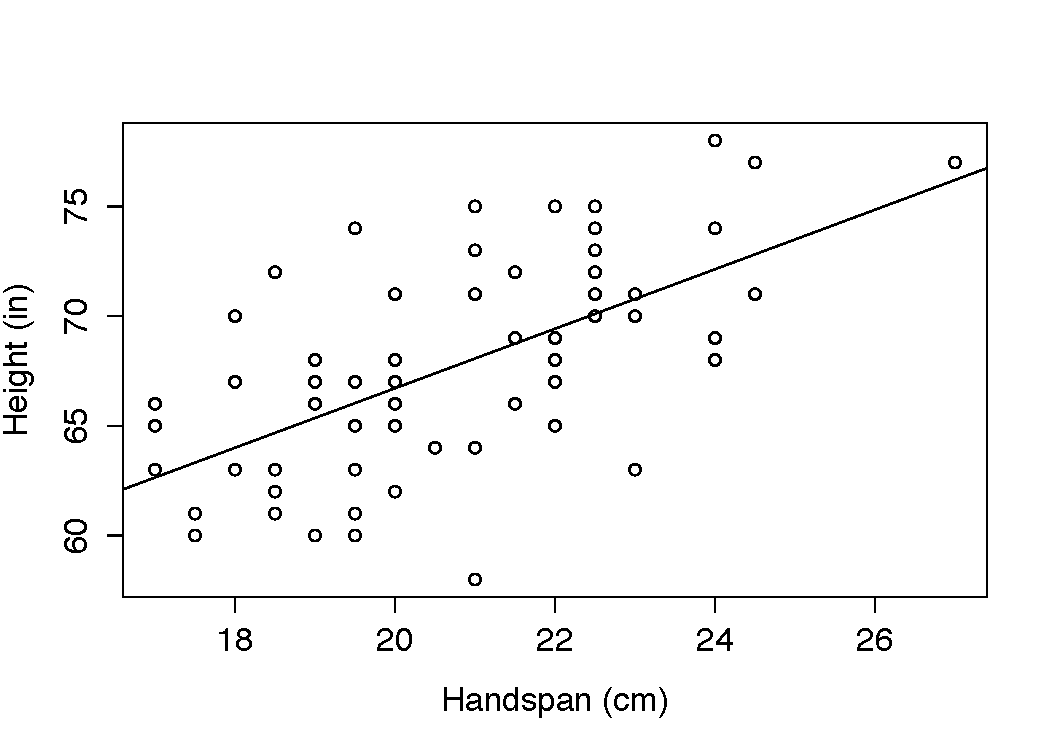
\includegraphics[scale = 0.3]{./images/height_handspan_reg}
\end{center}
The estimated slope was about 1.4 inches/cm and the estimated intercept was about 40 inches. \\


\alert{What if anything does this tell us about the relationship between height and handspan \emph{in the population}?}
\end{frame}
%%%%%%%%%%%%%%%%%%%%%%%%%%%%%%%%%%%%%%%%
\begin{frame}
	\frametitle{The Population Regression Model}
	How is $Y$ (height) related to $X$ (handspan) in the population?
	\begin{block}{Assumption I: Linearity}
		The random variable $Y$ is linearly related to $X$ according to 
			$$Y = \beta_0 + \beta_1 X + \epsilon$$
		$\beta_0,\beta_1$ are two unknown population parameters (constants).
	\end{block}

	\begin{block}
		{Assumption II: Error Term $\epsilon$}
		$E[\epsilon]=0$, $Var(\epsilon) = \sigma^2$ and $\epsilon$ is indpendent of $X$. The error term $\epsilon$ measures the unpredictability of $Y$ \emph{after controlling for $X$}
	\end{block}
\end{frame}
%%%%%%%%%%%%%%%%%%%%%%%%%%%%%%%%%%%%%%%%
\begin{frame}
	\frametitle{Predictive Interpretation of Regression}
	\begin{block}
		{Under Assumptions I and II}
		$$E[Y|X] = \beta_0 + \beta_1 X$$ 
			\begin{itemize}
				\item ``Best guess'' of $Y$ having observed $X=x$ is $\beta_0 + \beta_1 x$
				\item If $X = 0$, we predict $Y = \beta_0$
				\item If two people differ by one unit in $X$, we predict that they will differ by $\beta_1$ units in $Y$.
			\end{itemize}
	\end{block}
	\alert{The only problem is, we don't know $\beta_0, \beta_1$...}
\end{frame}
%%%%%%%%%%%%%%%%%%%%%%%%%%%%%%%%%%%%%%%%
\begin{frame}
	\frametitle{Estimating $\beta_0, \beta_1$}
Suppose we observe an iid sample $(Y_1, X_1), \hdots, (Y_n, X_n)$ from the population: $Y_i = \beta_0 + \beta_1 X_i + \epsilon_i$. Then we can \emph{estimate} $\beta_0, \beta_1$:

	$$\widehat{\beta}_1 = \frac{\sum_{i=1}^n (X_i - \bar{X}_n) (Y_i - \bar{Y}_n)}{\sum_{i=1}^n (X_i - \bar{X}_n)^2}$$

	
	$$\widehat{\beta}_0 = \bar{Y}_n - \widehat{\beta}_1 \bar{X}_n$$

\vspace{2em}
	\alert{Once we have estimators, we can think about sampling uncertainty...}
\end{frame}

%%%%%%%%%%%%%%%%%%%%%%%%%%%%%%%%%%%%%%%%

\begin{frame}
\frametitle{Sampling Uncertainty: Pretend the Class is our Population}

\begin{figure}[h]
\centering
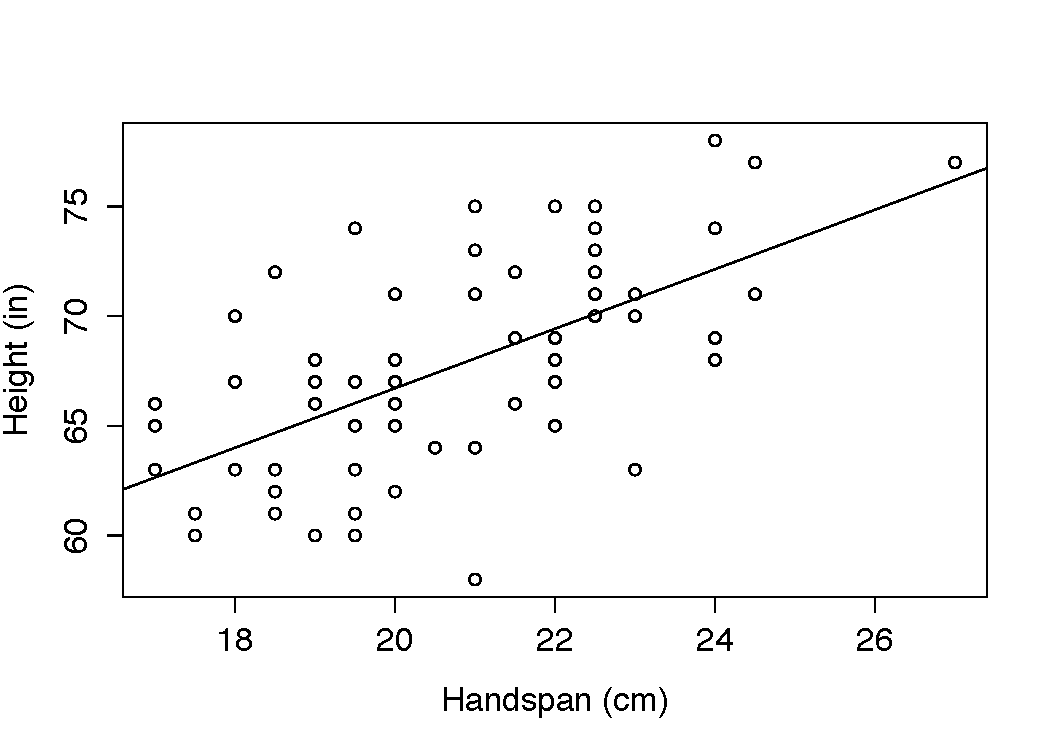
\includegraphics[scale = 0.5]{./images/height_handspan_reg}
\caption{Estimated Slope = 1.4, Estimated Intercept = 40}
\end{figure}


\end{frame}
%%%%%%%%%%%%%%%%%%%%%%%%%%%%%%%%%%%%%%%%
\begin{frame}
\frametitle{Sampling Distribution of Regression Coefficients $\widehat{\beta}_0$ and $\widehat{\beta}_1$}
\vspace{1em}

\begin{center}
\setlength{\unitlength}{1cm}
\begin{picture}(5,7)
\put(-2,6){\framebox(9,1){Choose 25 Students from Class List with Replacement}}



\put(0.5,6){\vector(-1,-1){1.5}}
\put(-2.3,3.7){\framebox(2.5,0.65){Sample 1}}



\put(-1,3.5){\vector(0,-1){1}}
\put(-1.6,1.9){\makebox{\small $\widehat{\beta}_0^{(1)}, \widehat{\beta}_1^{(1)}$}}



\put(2,6){\vector(0,-1){1.5}}
\put(0.7,3.7){\framebox(2.5,0.65){Sample 2}}



\put(2,3.5){\vector(0,-1){1}}
\put(1.4,1.9){\makebox{\small $\widehat{\beta}_0^{(2)}, \widehat{\beta}_1^{(2)}$}}



\put(3.8,4){\makebox{...}}
\put(3.8,2){\makebox{...}}



\put(4.5,6){\vector(1,-1){1.5}}
\put(4.8,3.7){\framebox(2.5,0.65){Sample 1000}}



\put(6,3.5){\vector(0,-1){1}}
\put(5.3,1.9){\makebox{\small $\widehat{\beta}_0^{(1000)}, \widehat{\beta}_1^{(1000)}$}}



\put(-2,0.6){\makebox{\small Repeat 1000 times $\rightarrow$  get 1000 different pairs of estimates}}



\put(-2,0.1){\makebox{\small \alert{Sampling Distribution: long-run relative frequencies}}}

\end{picture}
\end{center}


\end{frame}


%%%%%%%%%%%%%%%%%%%%%%%%%%%%%%%%%%%%%%%%

\begin{frame}
\frametitle{1000 Replications, $n=25$}

\begin{figure}[h]
\centering
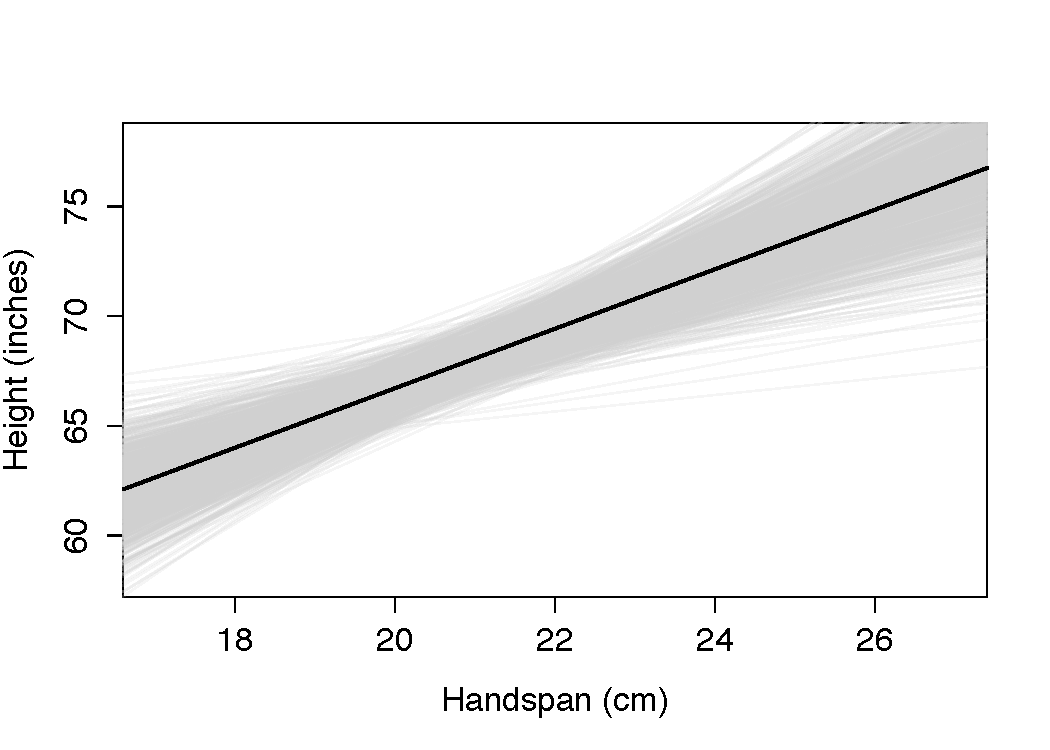
\includegraphics[scale = 0.6]{./images/reg_lines_sim}

\end{figure}


\end{frame}

%%%%%%%%%%%%%%%%%%%%%%%%%%%%%%%%%%%%%%%%

\begin{frame}
\frametitle{Population: Intercept = 40, Slope = 1.4}

\begin{figure}[h]
\centering
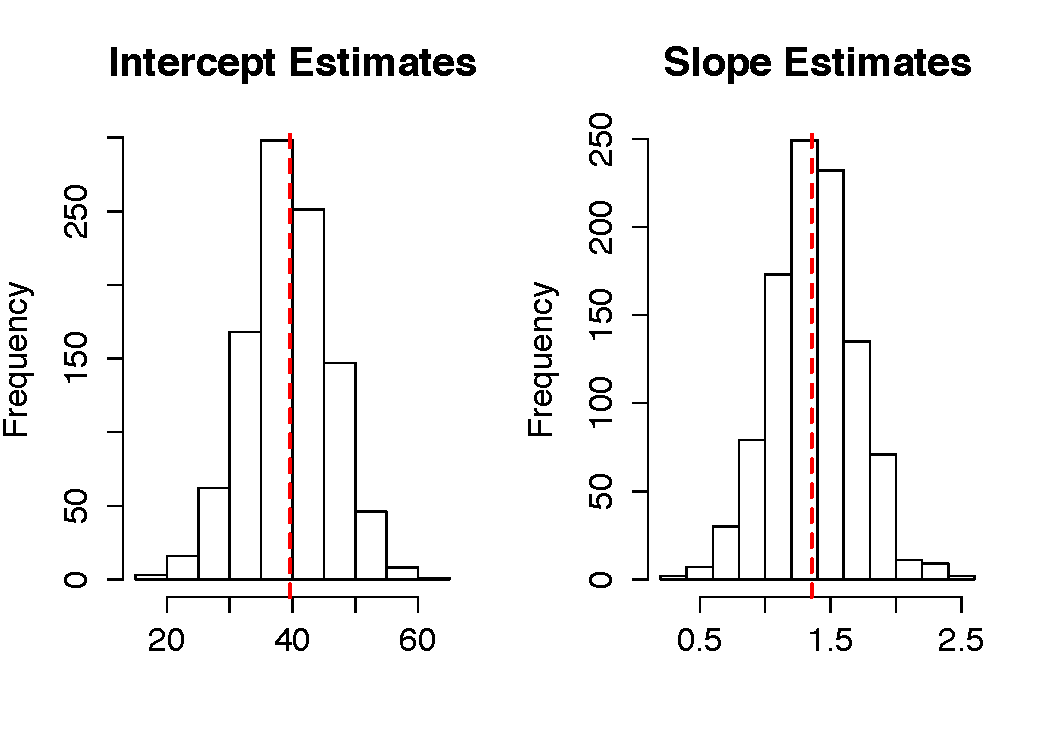
\includegraphics[scale = 0.55]{./images/reg_sim_hist}

\end{figure}
\alert{Based on 1000 Replications, $n = 25$}

\end{frame}

%%%%%%%%%%%%%%%%%%%%%%%%%%%%%%%%%%%%%%%%
\begin{frame}
\frametitle{Inference for Linear Regression}
	\begin{block}{Central Limit Theorem}
		$$\frac{\widehat{\beta} - \beta}{\widehat{SE}(\widehat{\beta})} \approx N(0,1)$$ 
\end{block}

\begin{block}{How to calculate $\widehat{SE}$?}
	\begin{itemize}
\item Complicated 
	\begin{itemize}
\item Depends on variance of errors $\epsilon$ and all predictors in regression. 
\item We'll look at a few simple examples 
\item R does this calculation for us 
\end{itemize}
\item Requires assumptions about population errors $\epsilon_i$ 
	\begin{itemize}
\item Simplest (and R default) is to assume $\epsilon_i \sim iid (0,\sigma^2)$ 
\item Weaker assumptions in Econ 104 
\end{itemize}

\end{itemize}
\end{block}

\end{frame}
%%%%%%%%%%%%%%%%%%%%%%%%%%%%%%%%%%%%%%%%
\begin{frame}
\frametitle{Intuition for What Effects $SE(\widehat{\beta}_1)$ for Simple Regression}

	$$SE(\widehat{\beta}_1) \approx \frac{\sigma}{\sqrt{n}} \cdot \frac{1}{s_X}$$
	\begin{itemize}
	\item $\sigma = SD(\epsilon)$ -- inherent variability of the $Y$, even after controlling for $X$
	\item $n$ is the sample size
	\item $s_X$ is the sampling variability of the $X$ observations.
	\end{itemize}
\end{frame}


%%%%%%%%%%%%%%%%%%%%%%%%%%%%%%%%%%%%%%%%
\begin{frame}
I treated the class as our population for the purposes of the simulation experiment but it makes more sense to think of the class as a sample from some population. We'll take this perspective now and think about various inferences we can draw from the height and handspan data using regression.
\end{frame}




%%%%%%%%%%%%%%%%%%%%%%%%%%%%%%%%%%%%%%%%
\begin{frame}[fragile]
\frametitle{Height = $\beta_0 +  \epsilon$}
\footnotesize
\begin{verbatim}
lm(formula = height ~ 1, data = student.data)
            coef.est coef.se
(Intercept) 67.74     0.51  
---
n = 80, k = 1
\end{verbatim}
\pause
\begin{verbatim}
> mean(student.data$height)
[1] 67.7375
\end{verbatim}
\pause
\begin{verbatim}
> sd(student.data$height)/sqrt(length(student.data$height))
[1] 0.5080814
\end{verbatim}
\end{frame}

%%%%%%%%%%%%%%%%%%%%%%%%%%%%%%%%%%%%%%%%
\begin{frame}
\frametitle{Dummy Variable (aka Binary Variable)}
 
A predictor variable that takes on only two values: 0 or 1. Used to represent two categories, e.g.\ Male/Female.
\end{frame}


%%%%%%%%%%%%%%%%%%%%%%%%%%%%%%%%%%%%%%%%

\begin{frame}[fragile]
\frametitle{Height = $\beta_0 + \beta_1$ Male $+ \epsilon$}

\footnotesize
\begin{verbatim}
lm(formula = height ~ sex, data = student.data)
            coef.est coef.se
(Intercept) 64.46     0.56  
sexMale      6.10     0.76  
---
n = 80, k = 2
residual sd = 3.38, R-Squared = 0.45
\end{verbatim}
\pause
\begin{verbatim}
> mean(male$height) - mean(female$height)
[1] 6.09868
\end{verbatim}
\pause
\begin{verbatim}
> sqrt(var(male$height)/length(male$height) +
		 			var(female$height)/length(female$height))
[1] 0.7463796
\end{verbatim}
\end{frame}


%%%%%%%%%%%%%%%%%%%%%%%%%%%%%%%%%%%%%%%%


\begin{frame}[fragile]
\frametitle{Height = $\beta_0 + \beta_1$ Male $+ \epsilon$ \hfill 
\includegraphics[scale = 0.05]{./images/clicker}}

\alert{What is the ME for an approximate 95\% confidence interval for the difference of population means of height: (men - women)?}

\footnotesize
\begin{verbatim}
lm(formula = height ~ sex, data = student.data)
            coef.est coef.se
(Intercept) 64.46     0.56  
sexMale      6.10     0.76  
---
n = 80, k = 2
residual sd = 3.38, R-Squared = 0.45
\end{verbatim}

\end{frame}


%%%%%%%%%%%%%%%%%%%%%%%%%%%%%%%%%%%%%%%%



\begin{frame}[fragile]
\frametitle{Height = $\beta_0 + \beta_1$ Handspan $+ \epsilon$}
\footnotesize
\begin{verbatim}
lm(formula = height ~ handspan, data = student.data)
            coef.est coef.se
(Intercept) 39.60     3.96  
handspan     1.36     0.19  
---
n = 80, k = 2
residual sd = 3.56, R-Squared = 0.40
\end{verbatim}

\end{frame}
%%%%%%%%%%%%%%%%%%%%%%%%%%%%%%%%%%%%%%%%
\begin{frame}[fragile]
\frametitle{Height = $\beta_0 + \beta_1$ Handspan $+ \epsilon$ \hfill 
\includegraphics[scale = 0.05]{./images/clicker}}
\alert{What is the ME for an approximate 95\% CI for $\beta_1$?}
\footnotesize
\begin{verbatim}
lm(formula = height ~ handspan, data = student.data)
            coef.est coef.se
(Intercept) 39.60     3.96  
handspan     1.36     0.19  
---
n = 80, k = 2
residual sd = 3.56, R-Squared = 0.40
\end{verbatim}
\end{frame}

%%%%%%%%%%%%%%%%%%%%%%%%%%%%%%%%%%%%%%%%
\begin{frame}
\frametitle{Simple vs.\ Multiple Regression}
\begin{block}{Terminology}
$Y$ is the ``outcome'' and $X$ is the ``predictor.''
\end{block}

\begin{block}{Simple Regression}
One predictor variable: $Y_i = \beta_0 + \beta_1 X_i + \epsilon_i$
\end{block}
\begin{block}{Multiple Regression}
More than one predictor variable: $Y_i = \beta_0 + \beta_1 X_{i1} + \beta_2 X_{i2} +  \hdots + \beta_k X_{ik} + \epsilon_i$
\end{block}


\begin{itemize}
	\item In both cases $\epsilon_1, \epsilon_2, \hdots, \epsilon_n \sim \mbox{iid} (0,\sigma^2)$
	\item Multiple regression coefficient estimates $\widehat{\beta}_1, \widehat{\beta}_1, \hdots, \widehat{\beta}_k$ calculated by minimizing  sum of squared vertical deviations, but formula requires linear algebra so we won't cover it.
\end{itemize}
\end{frame}

%%%%%%%%%%%%%%%%%%%%%%%%%%%%%%%%%%%%%%%%

\begin{frame}
\frametitle{Interpreting Multiple Regression}

\begin{block}{Predictive Interpretation}
$$Y_i = \beta_0 + \beta_1 X_{i1} + \beta_2 X_{i2} +  \hdots + \beta_k X_{ik} + \epsilon_i$$

$\beta_j$ is the difference in $Y$ that we would predict between two individuals who differed by one unit in predictor $X_j$ \emph{\alert{but who had the same values for the other $X$ variables.}} 

\end{block}

\begin{block}{What About an Example?}
	In a few minutes, we'll work through an extended example of multiple regression using real data.
\end{block}
\end{frame}

%%%%%%%%%%%%%%%%%%%%%%%%%%%%%%%%%%%%%%%%
\begin{frame}
\frametitle{Inference for Multiple Regression}

In addition to estimating the coefficients $\widehat{\beta}_0, \widehat{\beta}_1, \hdots, \widehat{\beta}_k$ for us, R will calculate the corresponding standard errors. It turns out that
	$$\frac{\widehat{\beta}_j - \beta_j}{\widehat{SE}(\widehat{\beta})} \approx N(0,1)$$
for \emph{each} of the $\widehat{\beta}_j$ by the CLT provided that the sample size is large.

\end{frame}
%%%%%%%%%%%%%%%%%%%%%%%%%%%%%%%%%%%%%%%%

\begin{frame}[fragile]
\frametitle{Height = $\beta_0 + \beta_1$ Handspan $+ \epsilon$}
\alert{What are \texttt{residual sd} and \texttt{R-squared}?}
\footnotesize
\begin{verbatim}
lm(formula = height ~ handspan, data = student.data)
            coef.est coef.se
(Intercept) 39.60     3.96  
handspan     1.36     0.19  
---
n = 80, k = 2
residual sd = 3.56, R-Squared = 0.40
\end{verbatim}
\end{frame}
%%%%%%%%%%%%%%%%%%%%%%%%%%%%%%%%%%%%%%%%

\begin{frame}
\frametitle{Fitted Values and Residuals}

\begin{block}{Fitted Value $\widehat{y}_i$}
Predicted $y$-value for person $i$ given her $x$-variables using estimated regression coefficients: \alert{$\widehat{y}_i = \widehat{\beta}_0 + \widehat{\beta}_1 x_{i1} + \hdots + \widehat{\beta}_k x_{ik}$}
\end{block}


\begin{block}{Residual $\widehat{\epsilon}_i$}
  Person i's \emph{vertical deviation} from regression line: \alert{$\widehat{\epsilon}_i = y_i - \widehat{y}_i$}. 
\end{block}

\vspace{1em}
\alert{The residuals are \emph{stand-ins} for the unobserved errors $\epsilon_i$.}

\end{frame}
%%%%%%%%%%%%%%%%%%%%%%%%%%%%%%%%%%%%%%%%
\begin{frame}
\frametitle{Residual Standard Deviation: $\widehat{\sigma}$}
	\begin{itemize}
    \item Idea: use residuals $\widehat{\epsilon}_i$ to estimate $\sigma$
	$$\widehat{\sigma}  = \sqrt{\frac{\sum_{i=1}^n \widehat{\epsilon}_i^2}{n -k}}$$ 
		\item Measures avg.\ distance of $y_i$ from regression line.
				\begin{itemize}
					\item E.g.\ if $Y$ is points scored on a test and $\widehat{\sigma}=16$, the regression predicts to an accuracy of about 16 points. 
				\end{itemize}
	\item Same units as $Y$ (Exam practice: verify this) 
	\item Denominator  ($n-k$) = (\# Datapoints - \# of $X$ variables) 
	\end{itemize}

\end{frame}




%%%%%%%%%%%%%%%%%%%%%%%%%%%%%%%%%%%%%%%%
\begin{frame}
\frametitle{Proportion of Variance Explained: $R^2$}
\framesubtitle{aka Coefficient of Determination}
	\begin{eqnarray*}
		R^2 \approx 1 - \frac{\widehat{\sigma^2}}{s_y^2}
	\end{eqnarray*}
		\begin{itemize}
			\item $R^2$ = proportion of $Var(Y)$ 
        ``explained'' by the regression.
			\begin{itemize}
			\item Higher value $\implies$ greater proportion explained 
			\end{itemize}
			\item Unitless, between 0 and 1 
      \item Generally harder to interpret than $\widehat{\sigma}$, but\dots 
			\item \alert{For simple linear regression $R^2 = (r_{xy})^2$ and this where its name comes from!}
		\end{itemize}
\end{frame}


%%%%%%%%%%%%%%%%%%%%%%%%%%%%%%%%%%%%%%%%

\begin{frame}[fragile]
\frametitle{Height = $\beta_0 + \beta_1$ Handspan $+ \epsilon$}
\footnotesize
\begin{verbatim}
lm(formula = height ~ handspan, data = student.data)
            coef.est coef.se
(Intercept) 39.60     3.96  
handspan     1.36     0.19  
---
n = 80, k = 2
residual sd = 3.56, R-Squared = 0.40
> cor(student.data$height, student.data$handspan)^2
[1] 0.3954669
\end{verbatim}
\end{frame}


%%%%%%%%%%%%%%%%%%%%%%%%%%%%%%%%%%%%%%%%
\begin{frame}[fragile]
\frametitle{Which Gives Better Predictions: Sex (a) or Handspan (b)?}
\footnotesize
\begin{verbatim}
lm(formula = height ~ sex, data = student.data)
            coef.est coef.se
(Intercept) 64.46     0.56  
sexMale      6.10     0.76  
---
n = 80, k = 2
residual sd = 3.38, R-Squared = 0.45

lm(formula = height ~ handspan, data = student.data)
            coef.est coef.se
(Intercept) 39.60     3.96  
handspan     1.36     0.19  
---
n = 80, k = 2
residual sd = 3.56, R-Squared = 0.40
\end{verbatim}

\end{frame}
%%%%%%%%%%%%%%%%%%%%%%%%%%%%%%%%%%%%%%%%


\begin{frame}
\begin{center}
\Huge Bring Your Laptop Next Time: We'll be Using R
\end{center}

\end{frame}


%%%%%%%%%%%%%%%%%%%%%%%%%%%%%%%%%%%%%%%%


\end{document}


